% Section content template for individual Educative lessons
% This file contains the actual content for a specific section
% Generated from Educative API section content

% Section: Activity Diagram for the Amazon Locker Service
% Section ID: 6599789557055488
% Section Slug: activity-diagram-for-the-amazon-locker-service
% Generated: 2025-12-11T15:17:26.649365

Activity diagrams are a great way to visualize the flow of messages from one activity to another in the system. There can be different activity diagrams that we can create for our Amazon Locker system. In this lesson, we will create an activity diagram for the product pickup activity.

\subsection{Product pickup}\label{yVcQnueR1MZocyYOVvyo_}
\\
The states and actions involved in this activity diagram are provided below.

\subsubsection{States}\label{krLO8AZBmaHcN3jOyK2c3}

\begin{itemize}
\item
\protect\phantomsection\label{7pmZeMQC_GDDKmXXXNRcq}
\textbf{Initial state:} A customer who has ordered a product from Amazon comes to the Amazon Locker to pick it up.
\item
\protect\phantomsection\label{QAZOc_HXbb75VUiWPWt46}
\textbf{Final state:} The customer successfully gets the product or the system shows an incorrect code error.
\end{itemize}

\subsubsection{Actions}\label{usmkQLFP2wL8x9orbmki4}
\\
The customer arrives at the Amazon Locker and enters the code. The system validates the code and opens the locker.
\\
Based on the order above, the activity diagram of product pickup is given below:

\begin{figure}[htbp]
 \centering
 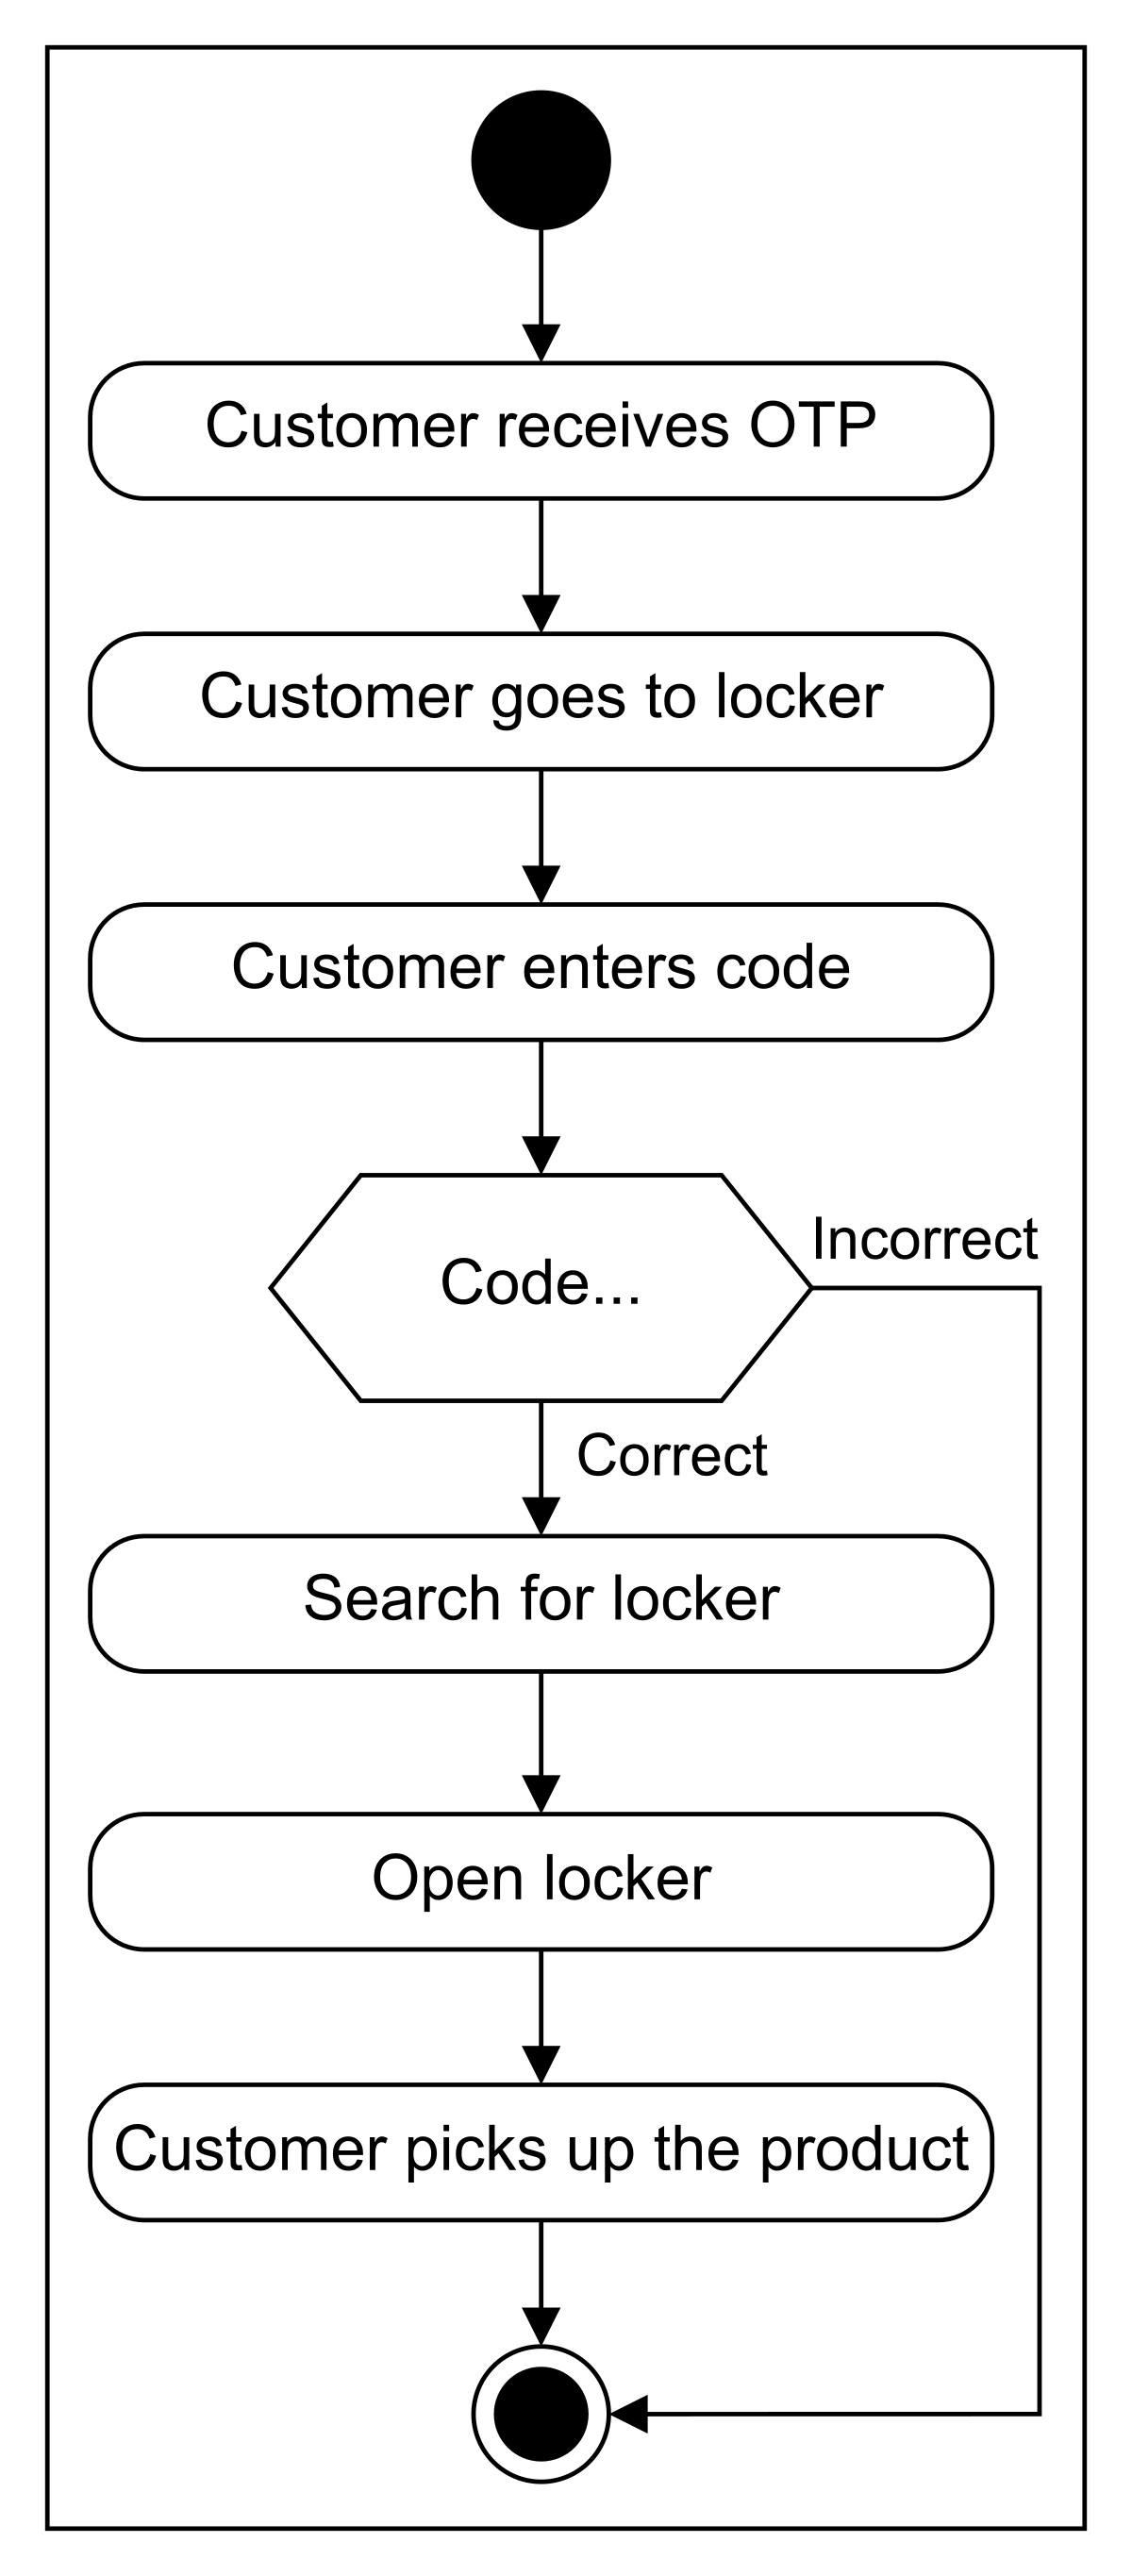
\includegraphics[width=0.5\textwidth]{Images/chapter_10/section_6599789557055488/5292277985312768.png}
 \caption{The activity diagram for product pickup from the locker}
\end{figure}

In the next lesson, we will present the code for our designed classes in some of the most popular languages.

% End of section content